\documentclass[useAMS,usenatbib]{mn2e}

% A Monthly Notices of the Royal Astronomical Society sample TeX file.
% The teX file has had all publication information removed and been left intentionally blank
% Created by: Martyn Bristow, M.Bristow@2007.ljmu.ac.uk, http://martynbristow.co.uk
% Edit this file to suit your needs, but be careful not to remove something important
% I have added sample images, tables and equations to help you if your don't know how to write them in LaTeX and to make your life easier.

\usepackage{graphicx}
\usepackage{float}
\usepackage{amsmath}
\usepackage{amssymb}
\usepackage{cite}
\usepackage{natbib}
\usepackage{xcolor}

\def\aap{Astronomy \& Astrophysics}
\def\apj{The Astrophysical Journal}
\def\mnras{Monthly Notices of the Royal Astronomical Society}

\usepackage{newtxtext,newtxmath}
\usepackage[T1]{fontenc}
\usepackage{ae,aecompl}
\usepackage{hyperref}

\newcommand{\red}[1]{{\color{red} #1}}

%%%%%%%%%%%%%%%%%%% TITLE PAGE %%%%%%%%%%%%%%%%%%%


\title[SL Challenge]{The Strong Gravitational  Lens Finding Challenge}

\author[R. B. Metcalf {\it et al.}]{
R. Benton Metcalf,$^{1,4}$\thanks{E-mail: robertbenton.metcalf@unibo.it} M. Meneghetti,$^4$ R\'emi Cabanac,$^2$ Emmanuel Bertin,$^3$ 
and  \\
% List of institutions
$^{1}$ Departimento di Fisica \& Astronomia, Universit\`a di Bologna, viale Berti Pichat 6/2, 40127 Bologna, Italy \\
$^{2}$ IRAP, University of Toulouse, CNRS, UPS, France.\\
$^{3}$ Sorbonne Universités, UPMC Univ. Paris 6 and CNRS, UMR 7095, Institut d'Astrophysique de Paris,  98bis Bd Arago, F-75014, Paris \\
$^{4}$ INAF-Osservatorio Astronomico di Bologna, via Ranzani 1, 40127 Bologna, Italy \\
}

\begin{document}

\date{Accepted . Received ; in original form }

\maketitle

\label{firstpage}

% Abstract of the paper
\begin{abstract}

\end{abstract}

\begin{keywords}
gravitational lensing -- cosmology 
\end{keywords}


\section{Introduction}

some numbers about future surveys

\section{The Challenge}

\section{the simulations}

\section{lens finding methods}

This section contains short descriptions of the lens finding methods that were used in 
the challenge.  Each subsection refers to a team which gave a separate entry.

\subsection{GAHEC IRAP (Remi Cabanac)}

\begin{figure}
 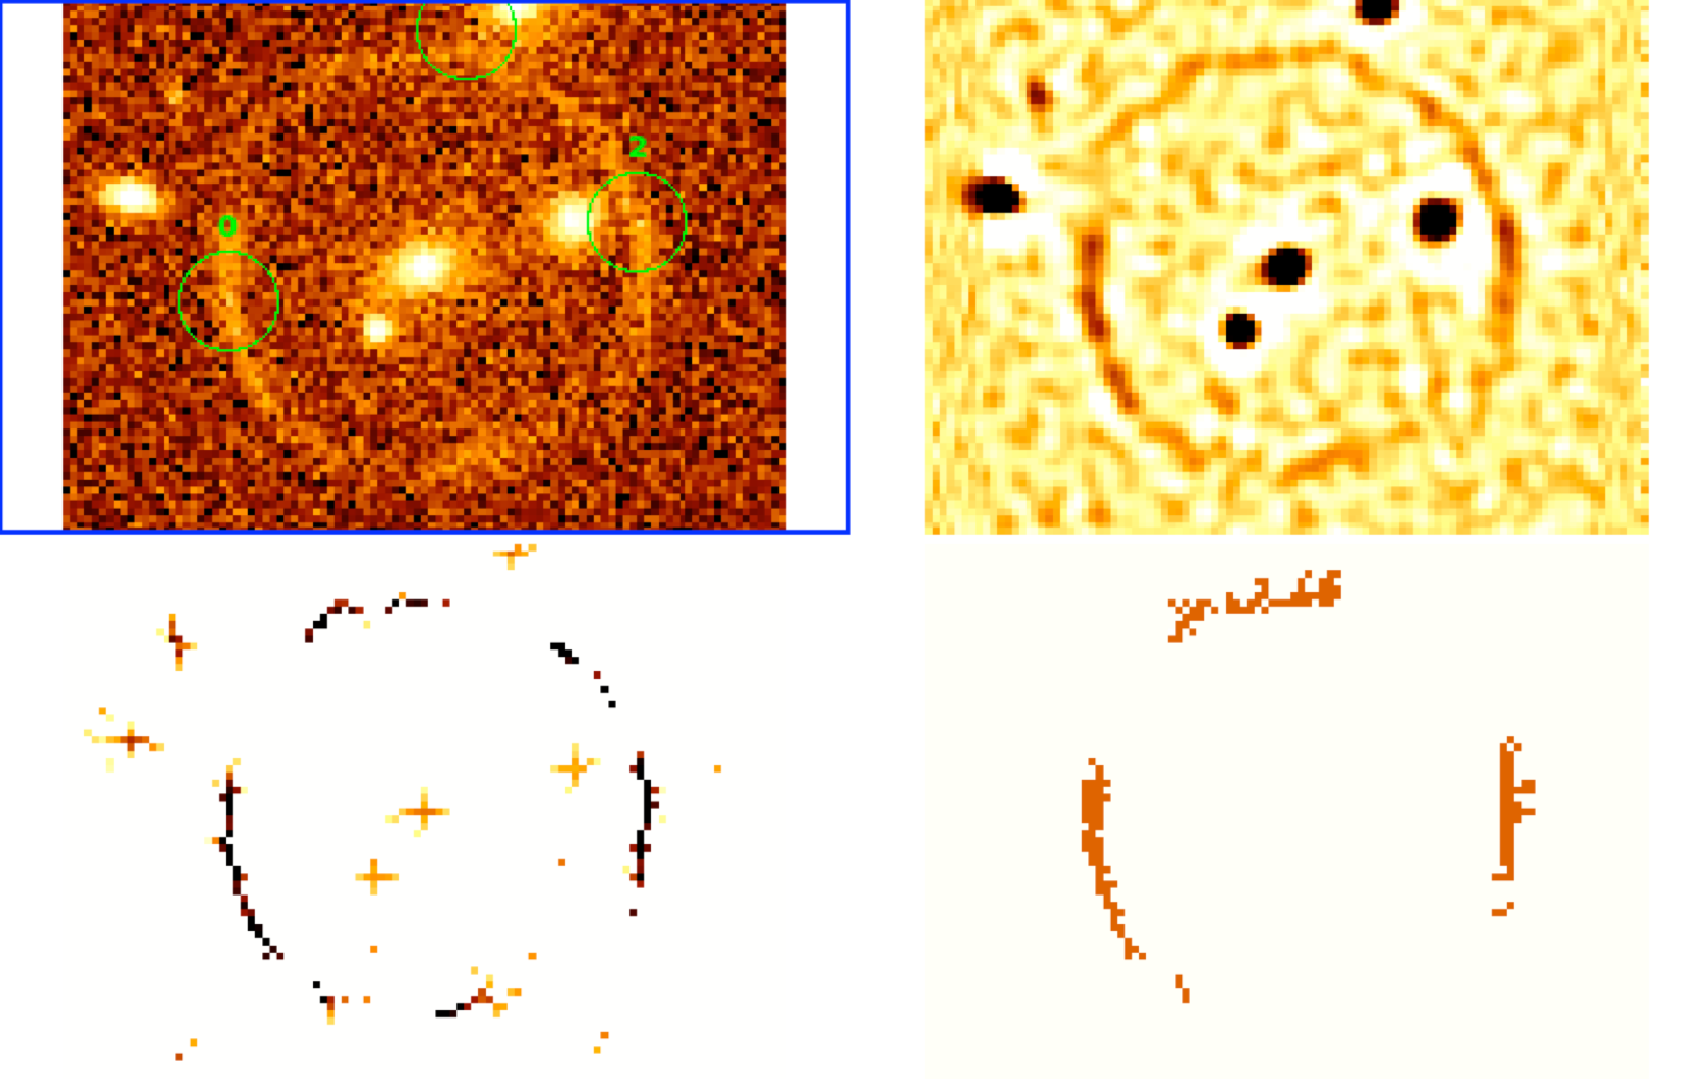
\includegraphics[width=\columnwidth]{Cabanac/arcmethod.pdf}
 \caption{ (GAHEC IRAP) From top-left to botton right, 1) a simulated arc extracted from SL challenge in which an tunned Arcfinder selects 3 candidates (green circles), 2) the smoothed image on which pixelwise elongation is computed, 3) the resulting elongated pixels after thresholding, 4) the set of pixels selected for the computation of arc candidate properties. }
 \label{fig:Cabanac}
\end{figure}

Arcfinder \citep{2006astro.ph..6757A,2007A&A...461..813C,2012ApJ...749...38M} is a fast linear method that computes a pixelwise elongation parameter (ratio of first-order moments in a n-pix window oriented in proper reference frame) for all pixels of mexican-hat-smoothed FITS images. Arcfinder then extract contiguous pixels above a given background and computes the candidate arcs length, width, area, radius of curvature and peak surface brightness. A final thresholding is set to maximize purity over completeness on a few typical arcs of the dataset.
For the current SL challenge, arcfinder was tunned to detect long and narrow arcs, and was optimized on a subset of 1000 simulated images with a grid covering a range of elongation windows and arc areas.  A python wrapper allows users to change parameters in a flexible way and run the arcfinder C code as a linux line command. Arcfinder took a couple of hours to run on the entire dataset with some overheads due to the dataset format. The code is publicly available at https://github.com/rcabanac/arcfinder.

\red{Reference to figure \ref{fig:Cabanac}?}

\subsection{AstrOmatic (Emmanuel Bertin)}

The lens detector is based on a convolutional neural network (CNN), trained with the provided training datasets. The CNN is implemented in Python, using the TensorFlow framework\footnote{http://www.tensorflow.org/}. Both ground multichannel and space monochannel image classifiers have the exact same CNN architecture.

The network itself consists of three convolutional layers ($11\times 11\times 32$, $5\times 5 \times 64$ and $3\times 3\times 64$), followed by two fully-connected layers ($256$ and $64$ neurons) and an output softmax layer. The first five layers use the ELU (Exponential Linear Unit) activation function \citep{2015arXiv151107289C}, which in our tests led to significantly faster convergence compared to ReLU and even SoftPlus activation. Dropout regularization \citep{2012arXiv1207.0580H,JMLR:v15:srivastava14a} is applied to both convolutional and fully connected layers, with ``keep'' probabilities $p=2/3$ and $p=1/2$, respectively.

Prior to entering the first convolutional layer, input image data are rescaled and dynamic-range compressed with function $f(x) =
\mathrm{arcsinh} (10^{11} x)$, and bad pixels are simply set to 0.
Data augmentation is performed in the form of random up-down and left-right image flipping, plus $k\pi/2$ rotations, where $k$ is a random integer in the $[0,3]$ range. Additionally, a small rotation with random angle $\theta$ is applied, involving bicubic image resampling. $\theta$ follows a Gaussian distribution with mean $\mu=0$ and standard deviation $\sigma_{\theta}=5^{\circ}$. No attempt was made to generate and randomize bad pixel masks in the data augmentation process.

The CNN weights are initialized to random values using a truncated Gaussian distribution with mean $\mu=0$ and standard deviation $\sigma=5.10^{-2}$. The network is trained on a Titan-X ``Pascal'' nVidia GPU using the Adam gradient-based optimizer \citep{2014arXiv1412.6980K} during 800 epochs, with an initial learning rate $\eta(t=0)=10^{-3}$ and a learning rate decay $\eta(t+1)/\eta(t)=0.99$, where $t$ is the epoch. Because of a lack of time, tests were limited to assessing the basic classification performance on a subset of the of 1,000 images/datacubes, using the 19,000 others for training.

\section{results}

\section{Conclusions \& discussion}

It is clear that the robustness of lens finders against falsely classifying unusual galaxies as lenses was not adequitely tested in this challenge.  Some of the methods which appear overly conservative in this test might be better at avoiding false positives in real data.  This can be seen as a form of overfitting to the test set.
In future challenges we wish to concentrate on this aspect of the problem.

Human inspection was the only method to find the jackpot lens

\section*{Acknowledgements}

EB thanks Raphael Gavazzi for proposing him to participate to the challenge.

%%%%%%%%%%%%%%%%%%%%%%%%%%%%%%%%%%%%%%%%%%%%%%%%%%
%%%%%%%%%%%%%%%%%%%% REFERENCES %%%%%%%%%%%%%%%%%%

\bibliographystyle{mn2e}
\bibliography{references}

%%%%%%%%%%%%%%%%%%%%%%%%%%%%%%%%%%%%%%%%%%%%%%%%%%
%%%%%%%%%%%%%%%%% APPENDICES %%%%%%%%%%%%%%%%%%%%%

\appendix

\label{lastpage}
\end{document}
